\section{Misión del sistema}

La implantación del AFUA tiene como objetivo proporcionar una mayor flexibilidad operativa a todos los usuarios del espacio aéreo mediante una configuración dinámica del mismo, que abarque todas las fases de la operación, desde la planificación inicial a la fase de análisis posterior a la operación, incluyendo la fase de ejecución.

Esta configuración dinámica nos permitirá reemplazar las distintas estructuras fijas utilizadas hasta ahora por volúmenes de espacio aéreo flexibles. Para conseguir esto, se debe tomar como piedra angular la coordinación civil–militar. Por lo que el primer objetivo del AFUA será conseguir que esta coordinación sea a través del ASM.

Los usuarios del espacio aéreo, civiles o militares, verán reflejada la implementación del AFUA de la siguiente manera:

\begin{itemize}
    \item \textbf{Militar.} La gestión dinámica del espacio aéreo permitirá una planificación y gestión de las operaciones militares mucho más cercana al periodo de operación en el caso de que sea necesario. La automatización proporcionada por las herramientas de soporte del ASM mejorará el proceso de decisión y aportará funcionalidades adicionales, como la capacidad de predicción de la situación a futuro, lo que mejorará la transparencia en las fases de ejecución y planificación.
    \item \textbf{Civil.} La gestión dinámica permitirá en este caso una mejorar planificación y gestión del balance necesario entre capacidad y demanda en los tres niveles de gestión.
\end{itemize}

En su objetivo de asegurar un uso óptimo del espacio aéreo disponible por todos los posibles usuarios, el AFUA hará imprescindible el desarrollo de un sistema de comunicaciones y apoyo en tiempo real. Este sistema permitirá mediante una continua actualización de una base de datos, con la información relativa a la fase de planificación y ejecución, que se establezca una coordinación directa entre los organismos locales de gestión civil y militar (AMC, ACC, etc) y el Network Manager.

De esta manera se mejorará la coordinación civil–militar y se tendrá un mayor conocimiento de la forma de operación de las distintas regiones de espacio aéreo. Además, esto permitirá aumentar la capacidad y reducir la carga de trabajo asociada a la fase de ejecución.

\subsection{Estructura organizacional del AFUA}

La estructura del AFUA, no es muy diferente de la del FUA, sino que utilizará herramientas y procedimientos más avanzados para lograr que el FUA proporcione estructuras del espacio aéreo más flexibles y eficientes. Por ello no se va a repetir la estructura ya expuesta en anteriores apartados sino que a continuación se van a exponer los cambios y mejoras respecto a ella. El AFUA introduce la siguiente serie de mejoras.

\subsubsection{Mejoras en la toma de decisiones}

Se realizará mediante \acrfull{cdm} que es el proceso mediante el cual todas las decisiones ATM, excepto las del ATC, se toman en base al intercambio de información relevante acerca de las operaciones entre los operadores civiles y militares.  

Mediante este proceso, la comunidad ATM comparte información necesaria para llevar a cabo las operaciones. Dicho intercambio de información posibilita la toma de decisiones, garantizando que las partes interesadas reciben información precisa y oportuna, esencial para la planificación de sus respectivas operaciones. Al permitir la toma de decisiones basada en información, se aumenta la previsibilidad en caso de eventos imprevistos o interrupciones, lo que permite hacer una utilización más óptima del espacio aéreo. El AFUA, pretende integrar la actividad del ATFCM, ASM y ATS utilizando el proceso de CDM, tal y como se muestra en la figura (\ref{fig:cdm}).

\begin{figure}[H]
    \centering
    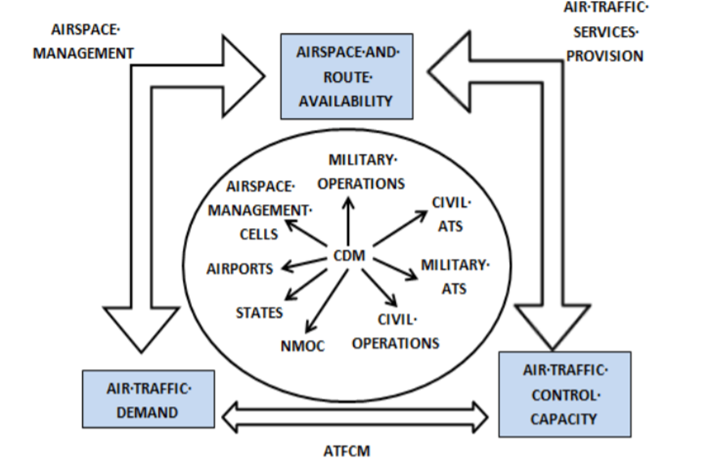
\includegraphics[width=1\linewidth]{figuras/cdm.png}
    \caption{Proceso CDM con las partes interesadas en el espacio aéreo.}
    \label{fig:cdm}
\end{figure}

\subsubsection{Trayectorias dinámicas y Free Routing}

Las operaciones de aeronaves civiles ya no se basarán en establecer un conjunto de rutas ATS fijas e invariables. El presente OCD introduce el concepto de trayectorias dinámicas que permitirán a las aeronaves, cambiar sus rutas en función de las actividades militares reservadas.  Los usuarios, sabrán en todo momento qué espacio aéreo está reservado para determinadas actividades. Dicha información les permitirá cambiar su ruta para evitar penetrar en dichos espacios aéreos. 

Este cambio se podrá realizar con la ayuda del concepto de Free Route, que permitirá a los usuarios del espacio aéreo tener más flexibilidad a la hora de elegir su trayectoria. 

\subsubsection{Mejoras en el intercambio de datos}

Para que todo lo mencionado anteriormente se pueda llevar a cabo de forma segura es necesario intercambiar gran cantidad de información entre lo operadores civiles y militares. Por esta razón es necesario disponer de un sistema capaz de ofrecer la información necesaria para que las operaciones se lleven a cabo de la manera más eficiente posible. Para ello es necesario el concepto de \acrfull{swim}, que será el sistema capaz de informar, notificar y dotar de más flexibilidad al sistema propuesto en el presente OCD.

\subsubsection{Uso de configuraciones de espacio aéreo}

El objetivo del AFUA, será reemplazar las estructuras fijas del espacio aéreo con volúmenes de espacio aéreo disponibles de forma dinámica. Este es uno de las evoluciones y cambios más grandes respecto el FUA. Las estructuras del FUA eran mucho más fijas y estáticas (ver apartado (\ref{tit:fua_estructura})) 

El AFUA utilizará las siguientes nuevas configuraciones:

\begin{enumerate}
    \item \textbf{Variable Profile Area (VPA)}
    
    Permite la asignación y gestión flexible de pequeños módulos fijos predefinidos de espacio aéreo. Su implementación permite una mejor respuesta a los requisitos y limitaciones militares y mejora la coordinación civil-militar, incluida la actualización del estado del espacio aéreo en tiempo real.

    \begin{figure}[H]
        \centering
        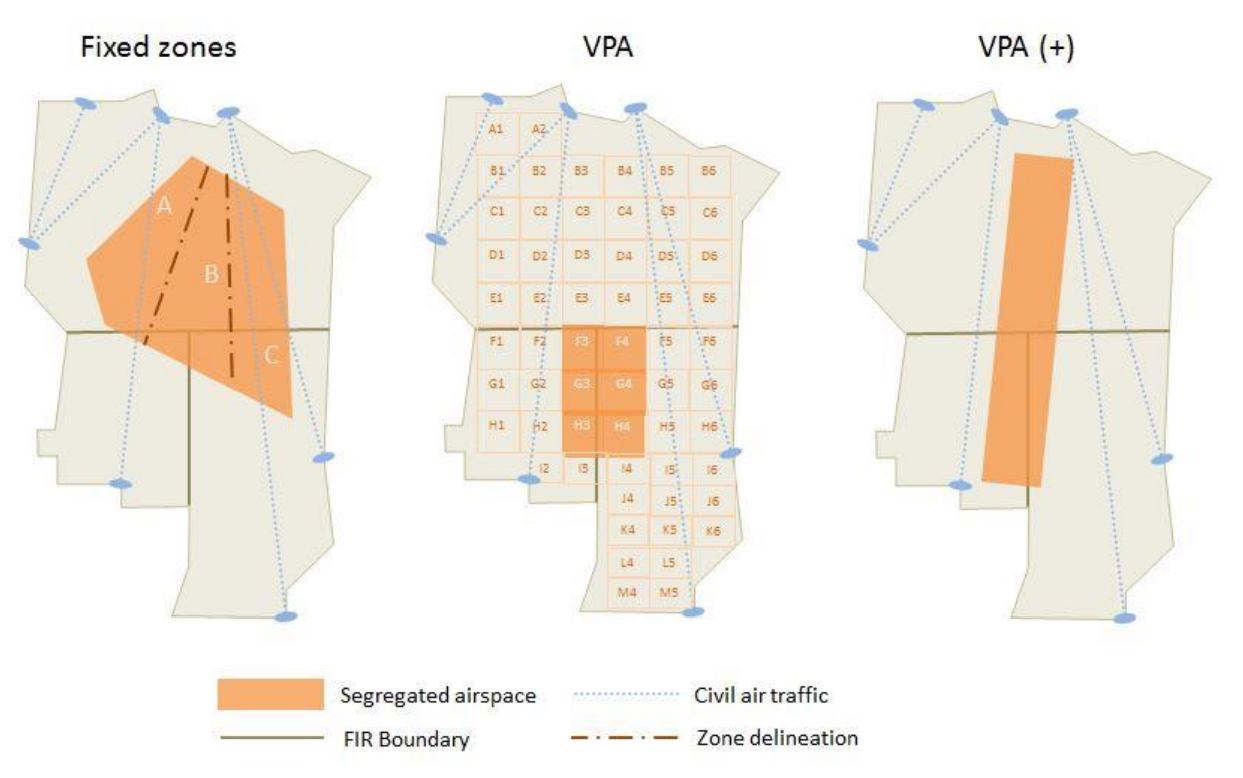
\includegraphics[width=1\linewidth]{figuras/vpa.png}
        \caption{Evolución de sectores fijos (FUA) a VPA (AFUA).}
        \label{fig:vpa}
    \end{figure}

    \item \textbf{Dynamic Mobile Area (DMA)}
    
    Son áreas destinadas al uso militar que permiten mejorar la flexibilidad del espacio aéreo. Se definen como un volumen de espacio aéreo en 4 dimensiones y se utiliza para proteger las actividades militares del tráfico civil. Existen tres tipos de DMAs:

    \begin{itemize}
        \item \textbf{Tipo 1:} son áreas definidas (dimensiones laterales y verticales) y asignadas (marco de tiempo de activación) para satisfacer las necesidades del usuario del espacio aéreo. La ubicación óptima del DMA se decide caso por caso. El AMC asignará un DMA en una ubicación específica para una misión determinada a fin de minimizar el impacto en el tráfico civil esperado.
        
        \begin{figure}[H]
            \centering
            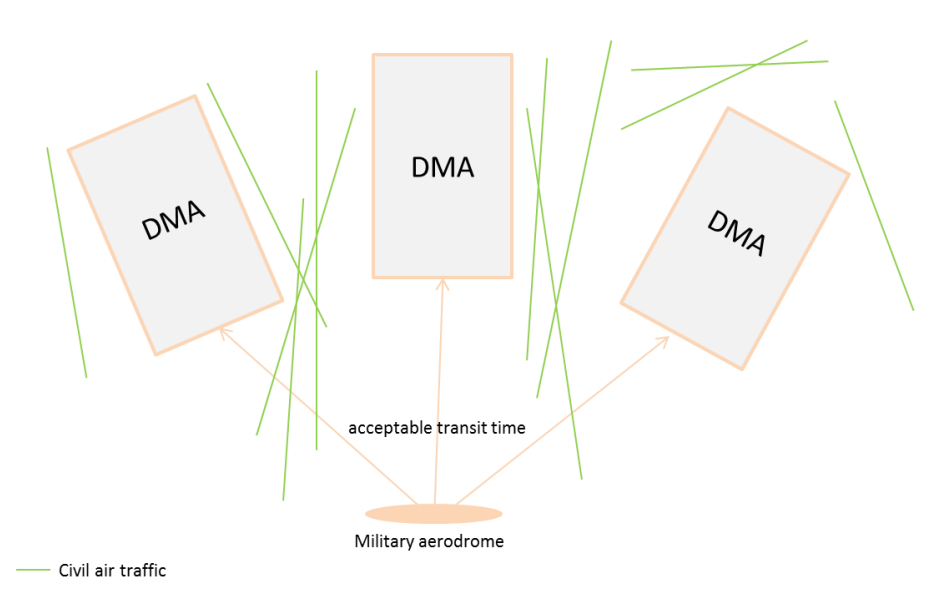
\includegraphics[width=0.8\linewidth]{figuras/dma_1.png}
            \caption{DMAs de tipo 1.}
            \label{fig:dma_1}
        \end{figure}
    
        \item \textbf{Tipo 2:} son áreas definidas con dimensiones laterales y verticales y asignación de tiempo de acuerdo con las necesidades del usuario del espacio aéreo. La diferencia con las DMAs del tipo 1 es que la ubicación del área cambiará a medida que ocurra la misión. Las misiones militares a menudo incluyen varias tareas en diferentes ubicaciones y diferentes niveles de vuelo (por ejemplo, reabastecimiento de combustible en el aire, ejercicios de combate, etc.). No siempre es posible asignar un área única que abarque todas estas tareas, ya que segregaría una parte importante del espacio aéreo y eso afectaría drásticamente los flujos de tráfico civil. 
        
        Los DMA de tipo 2 consisten en varias áreas más pequeñas definidas a lo largo de la trayectoria de la misión, que limitan el impacto en los flujos de tráfico civil y aseguran la asignación del espacio aéreo para los militares.
        
        \begin{figure}[H]
            \centering
            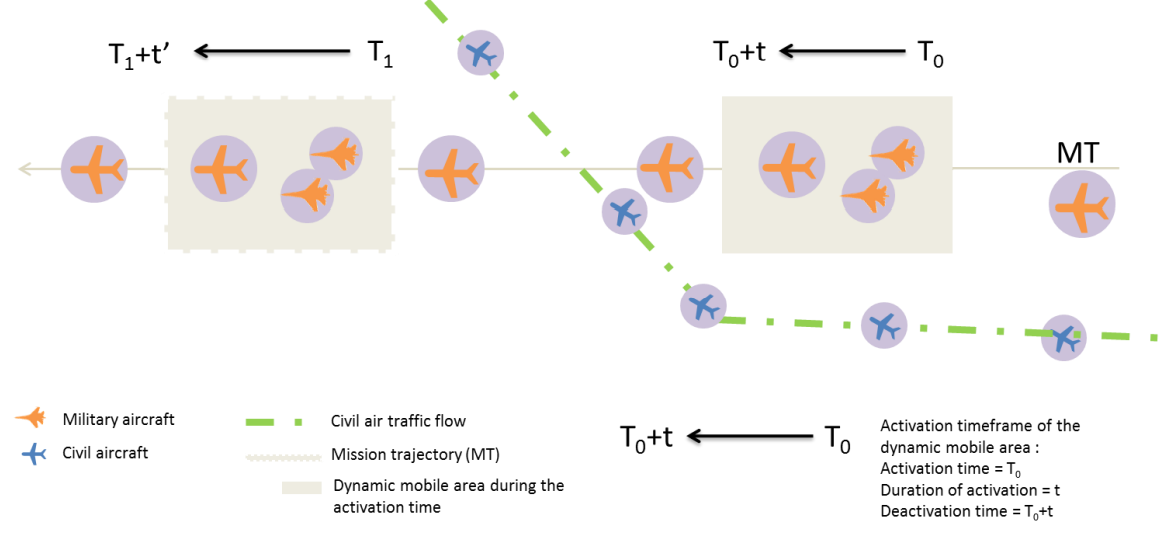
\includegraphics[width=0.8\linewidth]{figuras/dma_2.png}
            \caption{DMAs de tipo 2.}
            \label{fig:dma_2}
        \end{figure}
        
        \item \textbf{Tipo 3:} son áreas definidas con dimensiones laterales y verticales alrededor de actividades en movimiento que requieren una separación adecuada de las trayectorias de otros usuarios del espacio aéreo. Por lo tanto, los DMA de tipo 3 son burbujas que se mueven con el avión militar para separar el vuelo militar del resto del tráfico. Este tipo de DMA no solo minimiza la segregación del espacio aéreo, sino que también es beneficioso para el usuario del espacio aéreo militar al aumentar la flexibilidad. 
        
        \begin{figure}[H]
            \centering
            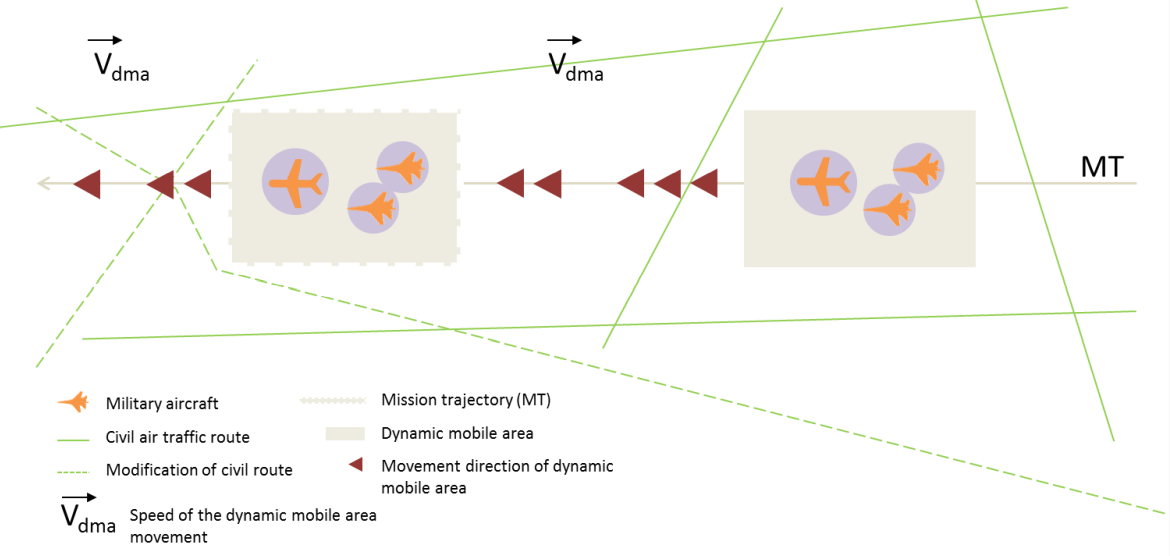
\includegraphics[width=0.8\linewidth]{figuras/dma_3.png}
            \caption{DMAs de tipo 3.}
            \label{fig:dma_3}
        \end{figure}
    \end{itemize}
\end{enumerate}

\subsection{Niveles de gestión. Estrategias}

Al igual que en el FUA, es necesario definir una serie de niveles que permitan gestionar las tareas relativas a la armonización y el conocimiento común de las medidas ASM/ATFCM y ATS.

En el caso del AFUA se distinguen 4 niveles como se puede ver en la figura (\ref{fig:niveles}):

\begin{figure}[H]
    \centering
    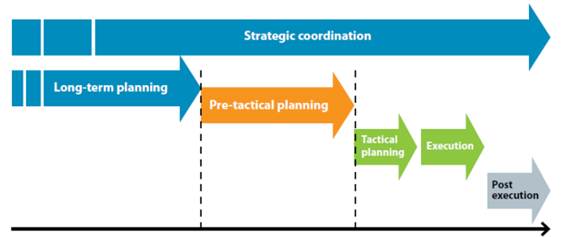
\includegraphics[width=1\linewidth]{figuras/niveles.png}
    \caption{Esquema de niveles de gestión y estrategias.}
    \label{fig:niveles}
\end{figure}

\subsubsection{Planificación estratégica}\label{tit:level1}

Comprende desde varios años antes de la operación hasta 7 días antes de la misma. La información relativa a las reservas de espacio aéreo orientadas a maniobras o ejercicios militares se conoce con antelación.

Se introducen un nuevo sistema que permite reservar regiones de espacio aéreo de manera provisional. Este sistema de reservas está específicamente diseñado para que dichas regiones de espacio aéreo puedan ser modificadas de acuerdo a las necesidades. 

\subsubsection{Fase pre-táctica}\label{tit:level2}

Comprende desde 7 días antes de la operación hasta el día de la misma. 
La información que se utiliza en esta fase para la planificación del espacio aéreo en los días posteriores está relacionada con los AUP’s (Airspace Use Plan) y UUP’s (Updated Airspace Use Plan) tanto a nivel nacional, como de bloque funcional (FAB’s) y del conjunto europeo de la red (EAUP y EUUP).

Además, contiene todas la actualizaciones necesarias acerca de la disponibilidad esperada de los CDR’s (Coded Departure Routes) y las reservas de espacio aéreo en el día de la operación.

\subsubsection{Fase táctica}\label{tit:level3}

Es la correspondiente al día de la operación.
La información utilizada es la relativa a la planificación a corto plazo y a la utilización del espacio aéreo en tiempo real.

Se define el status de las diferentes zonas de espacio aéreo como disponible, reservado, en uso o liberado. Proporciona información acerca de la forma y localización real de las porciones consideradas de espacio aéreo. 

Confirma lo definido en la fase pre-táctica relativo a la disponibilidad de los CDR’s y las reservas de espacio aéreo.

\subsubsection{Fase posterior a la operación}

Es una novedad respecto a lo planteado en el FUA. Tiene lugar el día posterior a la operación.
En esta fase la información está relacionada con las reservas y la utilización real que se dio a dichos espacios aéreos.

\subsection{Geografía y ubicación de las operaciones}

En el sistema AFUA que se pretende implantar en el espacio aéreo europeo, es clave la definición del proyecto del Cielo Único Europeo.

Dentro de la regulación asociada a este proyecto se hace hincapié en que todos los Estados miembros deben introducir todas las medidas necesaria para asegurar la implementación de los denominados bloques funcionales o \acrfull{fab}, que jugarán un papel clave en la implementación del AFUA.

Estos FAB, constituyen unos bloques de espacio aéreo basada en requisitos operacionales y establecidos sin tener en cuenta las fronteras entre Estados. En ellos, la provisión de servicios de navegación aérea y todas las funciones asociadas, están enfocados hacia la optimización de las actuaciones. 

En total, se han definido 9 iniciativas de bloques funcionales, como aparecen identificados en la figura (\ref{fig:fab}).

La introducción de estos bloques funcionales es clave en el desarrollo del AFUA, puesto que al eliminarse las fronteras nacionales, será más sencillo dirigir la definición de los espacios aéreos correspondientes con unas operaciones más optimizadas. 

El hecho de que los proveedores de navegación aérea trabajen de manera conjunta, permitirá flexibilizar los usos que se da al espacio aéreo en un marco de colaboración común.

\begin{figure}[H]
    \centering
    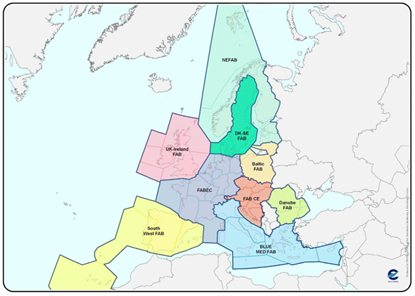
\includegraphics[width=0.8\linewidth]{figuras/fab.png}
    \caption{Bloques funcionales en Europa.}
    \label{fig:fab}
\end{figure}

Los objetivos que se marcan a la hora de definir los bloques funcionales son los siguientes:

\begin{itemize}
    \item Incrementar la seguridad.
    \item Aumentar la capacidad.
    \item Balancear los costes mediante una estructura más efectiva de rutas y provisión de servicios ATC.
    \item Conseguir una mayor eficiencia en las operaciones.
    \item Reducir el impacto sobre el entorno.
    \item Incrementar la efectividad de las operaciones militares.
\end{itemize}

En cuanto a su aplicación vertical, el AFUA se implementará en el espacio aéreo superior, es decir, por encima del FL195. La justificación de su implementación en el espacio aéreo superior viene dada por el hecho de que la coordinación de la parte civil y militar proporcionará más beneficios en los niveles de ruta de las aeronaves.

No hay que olvidarse de que el objetivo principal del sistema propuesto es evitar cambios de rutas debido a la segregación del espacio aéreo civil y militar. Esos cambios de trayectoria tendrán como resultado rutas más largas que llevan a incrementar el consumo de combustible en las aeronaves civiles y por tanto repercutirán de manera negativa en los costes y en el medioambiente. Por tanto, la aplicación del AFUA en esos niveles resulta indispensable para solucionar los problemas derivados de la segregación del espacio aéreo superior y proporcionar más flexibilidad dentro del mismo.

\begin{figure}[H]
    \centering
    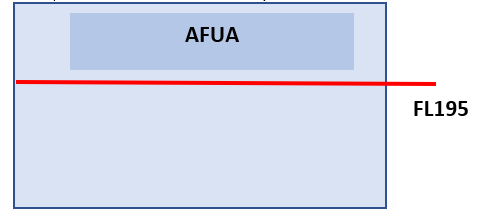
\includegraphics[width=0.8\linewidth]{figuras/afua_vertical.png}
    \caption{Aplicabilidad vertical del AFUA.}
    \label{fig:afua_vertical}
\end{figure}

\subsection{Sistemas relacionados}

A lo largo de este OCD ya han surgiendo varios sistemas que no solo están relacionados con el AFUA sino que son cruciales para que el concepto se pueda implementar y se convierta en un sistema real. En este apartado se van a listar dichos sistemas y hacer un pequeño resumen de ellos.

\subsubsection{System Wide Information Management (SWIM)}

El \acrfull{swim} son las normas, infraestructura y gobernanza que permiten la gestión de la información relacionada con el ATM y su intercambio entre partes cualificadas a través de servicios interoperables.

Dentro de SESAR se definen los siguientes principios clave  para el SWIM:

\begin{itemize}
    \item La información debe compartirse de forma segura en todo el sistema.
    \item La información pertinente estará disponible cuando y donde se necesite.
    \item La información se podrá personalizar, filtrar y acceder a ella, según sea necesario.
    \item El sistema incluirá todos los medidas de ciberseguridad necesarias para asegurar la confidencialidad, la integridad, la disponibilidad y la protección de los datos, las redes y los sistemas de control, la continuidad de las operaciones y las comunicaciones interoperables seguras.
    \item Autenticación para el acceso de los usuarios.
    \item La calidad inicial de la información será responsabilidad del emisor, la manipulación posterior no comprometerá su calidad.
    \item El intercambio de información puede ajustarse para mitigar cualquier problema de propiedad.
    \item La gestión de la información utilizará atributos de información armonizados a nivel mundial.
\end{itemize}

\subsubsection{Colaborative Decision Making (CDM)}

El \acrfull{cdm} es un proceso que sirve para apoyar otras actividades. Puede aplicarse a lo largo de la línea de tiempo de las actividades, desde la planificación estratégica (por ejemplo, las inversiones en infraestructuras) hasta las operaciones en tiempo real. El CDM no es un objetivo, sino una forma de alcanzar los objetivos de rendimiento de los procesos que apoya. Se espera que estos objetivos de rendimiento se acuerden en colaboración. 

Dado que la aplicación del CDM requerirá probablemente inversiones, éstas deberán justificarse de acuerdo con el enfoque basado en el rendimiento.

Aunque el intercambio de información es un factor importante, esto no es suficiente para realizar el CDM y sus objetivos. El CDM también requiere procedimientos y reglas predefinidos y acordados para garantizar que las decisiones de colaboración se tomen de forma rápida y equitativa.

El CDM garantiza que las decisiones se tomen de forma transparente, basándose en la mejor información disponible proporcionada por los participantes de forma oportuna y precisa.

El proceso para implementar el CDM en el AFUA o en cualquier otro sistema tiene las siguientes fases:

\begin{enumerate}
    \item Identificación de la necesidad del CDM.
    \item Análisis del CDM.
    \item Especificación y verificación del CDM.
    \item Caso de rendimiento del CDM.
    \item Validación y aplicación del CDM.
    \item Funcionamiento, mantenimiento y mejora del CDM. Esto es un proceso continuo.
\end{enumerate}

Es importante que los resultados de todas estas fases se compartan entre los miembros de la comunidad involucrados.

\subsubsection{Dynamic Airspace Configuration (DAC)}

\acrfull{dac} es un nuevo paradigma operativo que propone migrar del actual espacio aéreo estructurado y estático a un espacio aéreo dinámico capaz de adaptarse a la demanda de los usuarios al tiempo que satisface las cambiantes limitaciones de la meteorología, la congestión del tráfico y la complejidad, así como una flota de aviones muy diversa.

El DAC se ocupa de tres componentes principales: 

\begin{enumerate}
    \item La organización global del espacio aéreo.
    \item El cambio dinámico del espacio aéreo para satisfacer la demanda.
    \item Una caracterización genérica del espacio aéreo.
\end{enumerate}

El primer componente se refiere a la organización estratégica del espacio aéreo y a la creación de nuevas clases de espacio aéreo para aprovechar los conceptos y tecnologías que se espera que estén disponibles para 2025. 

El segundo componente se refiere a la reconfiguración dinámica del espacio aéreo necesaria para acomodar una demanda fluctuante. 

El tercer componente se refiere a los diseños "genéricos" del espacio aéreo que podrían promover la intercambiabilidad entre las instalaciones y los controladores mediante la eliminación de los componentes estructurales y funcionales del espacio aéreo que requerirían una formación específica del mismo.

\subsubsection{Free Route Airspace (FRA)}

\acrfull{fra} es un espacio aéreo especificado dentro del cual los usuarios pueden planificar libremente una ruta entre un punto de entrada y un punto de salida definidos. En función de la disponibilidad del espacio aéreo, la ruta puede planificarse directamente de uno a otro o a través de puntos de paso intermedios (publicados o no), sin referencia a la red de rutas ATS. Dentro de este espacio aéreo, los vuelos siguen estando sujetos al control del tráfico aéreo.

En un FRA el operador puede elegir su ruta con sólo algunas limitaciones (por ejemplo, puntos fijos de entrada y salida y la necesidad de evitar zonas de peligro, TRA o TSA), a diferencia de la situación en la que deben utilizarse las vías aéreas estándar. En la mayoría de los casos se elegirá la línea recta entre un punto de entrada y un punto de salida. 

Si por alguna razón esto no es apropiado (por ejemplo, hay que evitar una zona de peligro) se pueden especificar puntos de giro adicionales. Estos pueden ser ayudas a la navegación, puntos de navegación publicados o puntos con coordenadas especificadas.

La introducción de la FRA en Europa es un proceso gradual. La mayoría de los estados han decidido empezar con una implementación limitada (por ejemplo, durante las horas nocturnas) y luego ampliarla gradualmente.

A finales de 2020, 46 ACC habían implementado la FRA al menos parcialmente (pero en su mayoría sobre la base de H24). Además, hay muchas implementaciones transfronterizas, es decir, más de una ACC que participa en una iniciativa de FRA.